 
\documentclass[a4paper,12pt]{diplom}
% \usepackage[latin1]{inputenc}
% \usepackage[utf8]{inputenc}
\inputencoding{utf8} % Кодировка вашего файла


\usepackage{paratype} % Шрифты (можно отключить, если дает ошибку)
%% Немного увеличим шрифт в математическом режиме, чтобы соответствовать размерам Paratype-шрифтов
\DeclareMathSizes{12}{13.4}{11}{10}

\usepackage[left=3cm,right=2cm,top=2cm,bottom=2cm]{geometry} % Размеры полей
\usepackage[onehalfspacing]{setspace} % Полуторный интервал
%\renewcommand{\baselinestretch}{1.25} % Полуторный интервал
\usepackage{indentfirst} % Абзацный отступ в начале разделов
\setlength{\parindent}{1.25cm} % Величина абзацного отступа

\usepackage[pdftex]{graphicx} % Для вставки изображений
\usepackage{array} % Для таблиц
\usepackage{booktabs} % Для красивых таблиц 
\usepackage{tikz} % Рисунки с помощью TikZ
\usepackage[linesnumbered,lined,ruled]{algorithm2e} % Для оформления псевдокода
%\usepackage{algorithm} % Альтернатива оформления псевдокода
%\usepackage{algpseudocode} % Альтернатива оформления псевдокода
\usepackage{listings} % Оформление листингов программ
\usepackage{icomma} % Удаляем тонкий пробел после запятой в мат. режиме

% Если на нумерованную формулу нет ссылки в тексте,
\mathtoolsset{showonlyrefs} % то она становится ненумерованной

% microtype улучшает распределение символов в строке
\usepackage{microtype}  % Можно отключить, если возникают ошибки компиляции

% Формируем PDF с полноценными перекрестными ссылками
\usepackage[unicode, pdfborder={0 0 0}, pdfstartview=FitV]{hyperref}

% Часто используемые макросы
\newcommand{\N}{\mathbb{N}}  % Множество натуральных чисел
\newcommand{\Z}{\mathbb{Z}}  % Множество целых чисел
\newcommand{\R}{\mathbb{R}}  % Множество действительных чисел
\DeclareMathOperator{\sgn}{sgn} % Знак числа
\DeclareMathOperator{\M}{\mathsf{M}} % Матожидание
\newcommand{\from}{\colon} % Двоеточие в определении функции. Пример: $f \from \R \to \N$.
% Заменяем англоязычные обозначения на русские
\renewcommand{\le}{\leqslant}
\renewcommand{\leq}{\leqslant}
\renewcommand{\ge}{\geqslant}
\renewcommand{\geq}{\geqslant}
\renewcommand{\emptyset}{\varnothing}
\renewcommand{\epsilon}{\varepsilon}


%%%%%%%%%%%%%%%%%%%%%%%%%%
% Конец преамбулы
%%%%%%%%%%%%%%%%%%%%%%%%%%

\begin{document}

% Содержимое титульного листа

%\LetterHead{Минобр...}
\Kafedra{Кафедра информатики}

% Зав. кафедрой
\ZavKaf{Заведующий кафедрой,\\ д.\,ф.-м.\,н., профессор}{С.\,С.~Сидоров}
% Если это курсовая работа и виза зав. каф. не нужна, раскомментируйте следующую строку
%\Kursovaya

% Вид работы: Курсовая работа, Выпускная квалификационная работа, 
\DocumentType{\large Выпускная квалификационная работа}

% Название дипломной работы
\Title{\begin{Large}\bfseries Название дипломной работы\\ не помещающееся в одну строку\end{Large}}

% Направление подготовки
\Napr{по направлению\\ 02.03.02 Прикладная математика и информатика}

% Руководитель
\Chief{Научный руководитель\\ к.\,ф.-м.\,н., доцент}{И.\,И.~Иванов}

% Автор
\Author{Студент группы ИВТ-41БО}{И.\,И.~Иванов}

%\City{Ярославль}
%\Year{2017}


% Создаем титульный лист
\maketitle
\chapter{Реферат}

Объем \total{page} с., \total{chapternum} гл., \total{fignum} рис.,
\total{tablenum} табл., \total{bibnum} источников, \total{appnum} прил.

\medskip

Ключевые слова: \textbf{Алгоритм Бинарного разбиения, реабилитация, веб-приложения, процесс раз-
работки ПО.}

\medskip

Это пример оформления дипломной работы с помощью издательской системы \LaTeXe.

Реферат размещается непосредственно за титульным листом. Объем реферата должен составлять не более половины страницы. В~реферате указываются параметры ВКР: объем работы в страницах, количество глав, иллюстраций, таблиц, приложений, использованных источников. Перечень ключевых слов должен включать от~5 до~15 слов или словосочетаний из текста работы, которые в~наибольшей мере характеризуют ее содержание и~обеспечивают возможность информационного поиска. Ключевые слова приводятся в именительном падеже и~печатаются прописными буквами полужирным шрифтом в~строку через запятые.

Текст реферата должен отражать объект исследования, цель работы, результаты работы, область применения, степень внедрения или рекомендации по~внедрению.

% Содержание
\tableofcontents[Содержание]

% Пример ненумерованной главы
\chapternonum{Введение}

% Если исходное название содержит специальные символы (например, \\),
% то в квадратных скобках пишем упрощенный вариант названия для "Содержания".
\chapter[Длинное название очень длинное]{Длинное название \\ очень длинное}





Выпускная квалификационная работа включает следующие структурные элементы:
\begin{enumerate}[label=\arabic{enumi})]
	\item титульный лист;
	\item реферат;
	\item содержание;
	\item введение;
	\item основную часть:
	\begin{itemize}
		\item глава 1,
		\item глава 2,
		\item \dots;
	\end{itemize}
	\item заключение;
	\item список использованных источников (список литературы);
	\item приложения.
\end{enumerate}
Каждый структурный элемент ВКР начинается с новой страницы.

Разделы <<Введение>> и <<Заключение>> не нумеруются. 
В~них не~должно содержаться рисунков, формул и~таблиц.

Основная часть выпускной квалификационной работы не~требует специального заголовка, а~делится на~главы, состоящие из~параграфов, которые в~свою очередь, могут быть разбиты на~пункты. Каждая из~этих составляющих имеет заголовок, входящий в~состав содержания. Слова <<глава>>, <<параграф>>, <<пункт>> в~заголовках не~используются.  
Нумерация выше названных составляющих основной части производится по~числовой иерархической системе, причем после последней цифры, а~также после заголовка точка не~ставится.


\chapter{Оформление элементов текста}

\section{Рисунки и таблицы}
Иллюстрации (фотографии, рисунки, чертежи, графики, диаграммы и~т.\,п.) обозначаются сокращенно словом <<Рис.>>, которое пишется под иллюстрацией  с~прописной буквы и~выделяется полужирным шрифтом. Нумеруются иллюстрации арабскими цифрами. Нумерация сквозная по~всему тексту ВКР. Пример "--- рис.~\ref{fig:1}.
Под рисунком по~центру размещаются его наименование и~поясняющие надписи. 
Иллюстрации располагают сразу~же после ссылки на них в~тексте ВКР. 

% Рисунок
\begin{figure}[!ht]
	\centering
	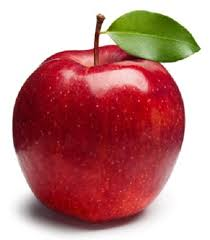
\includegraphics[width=0.3\textwidth]{apple.jpg}
	\caption{Название рисунка}
	\label{fig:1} % Метка для ссылки в тексте
\end{figure}

Таблицы нумеруются в рамках раздела  арабскими цифрами. Слово <<Таблица>> и~ее~номер пишется вверху, с~правой стороны над таблицей.
Ниже слова <<Таблица>>  посередине строки помещают ее название. Название  таблицы должно отражать ее~содержание, быть точным и~кратким. Название таблицы записывается с~прописной буквы и~выделяется полужирным шрифтом. Заголовки строк и~столбцов выделяются полужирным шрифтом.
Пример "--- табл.~\ref{tab:1}.

% Таблица
\begin{table}[tbh]
	\caption{Название таблицы}
	\label{tab:1} % Метка для ссылки в тексте
	\centering
	\begin{tabular}{lccc}
		\toprule
		& \multicolumn{3}{c}{\textbf{Число глав}}\\
		\cmidrule(l){2-4}
		\textbf{Тип работы} & \textbf{Одна} & \textbf{Две} & \textbf{Три} \\
		\midrule 
		Курсовая & 3 & 2 & 1 \\
		Работа бакалавра & 2 & 4 & 3 \\
		Диплом & 1 & 5 & 6 \\
		Магистерская диссертация & 0 & 4 & 5 \\
		\bottomrule
	\end{tabular}
\end{table}

\section{Заголовки и приложения}

\subsection{Заголовки}
Заголовки должны четко и кратко отражать содержание соответствующих разделов, подразделов, пунктов.
Заголовок печатают, отделяя от~номера пробелом, с~заглавной буквы. Точка в~конце заголовка не~ставится. 
Заголовки выделяют полужирным шрифтом.
В~заголовках следует избегать сокращений (за исключением общепризнанных аббревиатур). В~заголовке не~допускается перенос слова на~следующую строку и~подчеркивание слов.
Выравнивание заголовков выполняется по~левому краю или по~центру строки (единообразно во~всей работе) без абзацного отступа.
Расстояние между названием глав и~последующим текстом должно равняться двум межстрочным интервалам. Такое~же расстояние выдерживается между заголовками главы и~параграфа.

\subsection{Приложения}

В~виде приложений оформляется материал, дополняющий основную часть ВКР.  
Приложения обозначают прописными буквами русского алфавита, начиная с~А, за исключением букв Ё, З, Й, О, Ч, Ь, Ы, Ъ. 
Каждое приложение начинается с~новой страницы.  При~этом в~верхнем правом углу страницы приводят слово <<Приложение>>, записанное строчными буквами с~первой прописной, с~указанием номера приложения.  
Название приложения располагается ниже его обозначения на~отдельной строке по~центру  строчными буквами с~первой прописной и~выделяется полужирным шрифтом.
Приложения должны иметь общую с~основной частью документа сквозную нумерацию страниц.
В~тексте ВКР должны быть даны ссылки на~все приложения. 
Ссылки на~приложения в~тексте ВКР должны быть организованы в~строго нумерационном порядке.
Пример оформления "--- приложение~\ref{app:source}.

\section{Нумерация страниц}

Все страницы текста ВКР, включая его иллюстрации и~приложения, должны иметь сквозную нумерацию. 
Титульный лист считается страницей №~1, но~номер на~нем не~проставляется. 
Номера страниц проставляются арабскими цифрами внизу страницы в~ее~правом углу или по~центру. В~случае необходимости номер на~некоторых страницах может быть проставлен вручную.


\chapter{Формулы}

Издательская система \LaTeX~\cite{TeX:YarSU} предлагает широкий спектр средств для набора математических формул.
Подробно эта тема освещается в многочисленных книгах (см., например,~\cite{Oetiker:2016, Kotelnikov:2004}).
Ниже приводится лишь несколько простых примеров.

Если параметр~$a$ равен нулю, а~$b \ne 0$, то~уравнение \(a x = b\) не~имеет корней.

Определим функцию $\sgn \from \R \to \N$ следующим образом:
\begin{equation}
\sgn(x) = \begin{cases}
	 1, & \text{при } x \ge 0,\\
	-1, & \text{иначе.}
\end{cases}
\label{eq:sgn}
\end{equation}
Из формулы~\eqref{eq:sgn} следует, что $x \sgn(x) = |x|$.

\emph{Множество рациональных чисел:}
\[ 
	\mathbb{Q} \coloneqq \Set*{ \frac{n}{m} \given n\in\Z, \ m\in\N}.
\]

Вероятность события $A$ при условии, что событие~$B$ произошло:
$\Pb{A \given B}$.
% $\Prob$ "--- вероятность, $\Variance$ "--- дисперсия.

Вот так выглядит $(n\times k)$"~матрица:
\begin{equation}
M = \begin{pmatrix}
	m_{11} & m_{12} & \dots & m_{1k} \\
	m_{21} & m_{22} & \dots & m_{2k} \\
	\vdots & \vdots & \ddots & \vdots \\
	m_{n1} & m_{n2} & \dots & m_{nk} \\
	\end{pmatrix}
	\label{eq:matrix}
	% При наличии \mathtoolsset{showonlyrefs} в преамбуле
	% и отсутствии в тексте ссылок на метку eq:matrix
	% номер формулы не будет напечатан
\end{equation}


\chapter{Рисуем с помощью TikZ}

Пакет Ti\textit{k}Z предлагает удобные инструменты для рисования диаграмм, блок"=схем, графов, графиков функций и~т.\,п~\cite{tikz, Kirutenko:2014}.
При этом рисунки сохраняются в~векторной графике, а~для  надписей используется тот~же шрифт, что и~в~основном тексте.
Простейшие примеры использования этого пакета изображены на~рис.~\ref{fig:block} и~\ref{fig:sin}.


\usetikzlibrary{positioning} % Для конструкции right = of ...
\usetikzlibrary{arrows.spaced} % Для stealth'
\usetikzlibrary{calc} % Для $(...)!.5!(...)$
\usetikzlibrary{shapes.geometric} % Для diamond

\begin{figure}[ht]
	\begin{minipage}[b]{0.40\textwidth}
		\centering
		\begin{tikzpicture}[rect/.style={rectangle, thick, draw=black}, node distance=15mm and 10mm]
		\node (source) [draw=black, shape=diamond, shape aspect = 2, align=center] {Источник\\ данных};
		\node (result) [rect, rounded corners, right = of source] {Результат};
		\draw[->, >=stealth'] (source.north) to[bend left] (result);
		\node (C1) at ($(source.east)!.5!(result.west)$) {};
		\node (user) [draw=black, ellipse, below = of C1] {Наблюдатель};
		\draw[->, >=stealth'] (user.west) -| (source.south);
		\draw[<->, >=stealth'] (user) to (result);
		\end{tikzpicture}
		\caption{Блок-схема}\label{fig:block}
	\end{minipage}
	%
	\hfill% раздвигаем боксы по горизонтали
	%
	\begin{minipage}[b]{0.54\textwidth}
		\centering
		\begin{tikzpicture}[scale=1.0, >=stealth']
		%\draw[help lines] (-3.4,-1.3) grid[step=1.0] (3.8,1.3);
		\draw[->] (0, -1.3) -- (0, 1.5) node[right] {y};
		\draw[->] (-3.4, 0) -- (3.8, 0) node[above left] {x};
		\draw[thick, smooth, samples at = {-3.4,-3.2,...,3.8}] plot ({\x},{sin(\x*180/pi)});
		\draw[dashed] (0, 1.0) node[left] {1} -- (pi/2, 1.0) -- (pi/2, -0.05) node[below] {$\frac{\pi}{2}$};
		\node[below=0.1] at (pi, 0) {$\pi$};
		\node[below right] at (0, 0) {$O$};
		\end{tikzpicture} 
		\caption{График  функции $y = \sin(x)$} 
		\label{fig:sin}
	\end{minipage}
\end{figure}

\chapter{Псевдокод}

Пакет \href{https://www.ctan.org/pkg/algorithm2e}{algorithm2e}
предлагает широкий спектр инструментов для создания и оформления псевдокода.
Также имеется возможность делать ссылки на строки кода.
Например, в строке~\ref{alg:lDoWhile} алгоритма~\ref{alg:quicksort}
целиком содержится цикл типа \texttt{do-while}.

\SetAlgorithmName{Алгоритм}{Список алгоритмов}{} % Название на русском
\SetAlgoCaptionSeparator{.} % Отделяем название алгоритма от его номера точкой
%\SetAlgoLined % Вертикальные линии, соединяющие начало и конец блока
\DontPrintSemicolon % Не печатать точку с запятой
\SetKwProg{Proc}{Procedure}{}{end} % Команда для процедуры
\SetKwProg{Fn}{Function}{}{end} % Команда для функции
% Описание входных и выходных данных
\SetKwInOut{Input}{Вход}
\SetKwInOut{Output}{Выход}
\SetKwRepeat{DoWhile}{do}{while} % Создаем цикл do-while
\SetKwBlock{Loop}{loop}{endloop} % Безусловный цикл
\begin{algorithm}
	\caption{Быстрая сортировка} % Заголовок
	\label{alg:quicksort}
	% Обозначения ключевых (входных-выходных) данных алгоритма
	\SetKwArray{Array}{A} % Массив
	\SetKwData{Low}{b}
	\SetKwData{High}{e}
	% Названия новых процедур и функций
	\SetKwFunction{QuickSort}{QuickSort}
	\SetKwFunction{Partition}{Partition}
	% Описание входа-выхода
	\Input{ массив \Array, индексы начала \Low и конца \High сортируемого фрагмента}
	\Output{ массив \Array, отсортированный по возрастанию}
	\BlankLine
	% Непосредственно процедура QuickSort
	\Proc{\QuickSort{\Array, \Low, \High}}{
		\If{$\Low < \High$}{
			$m \leftarrow$ \Partition{\Array, \Low, \High}\;
			\QuickSort{\Array, \Low, $m$}\;
			\QuickSort{\Array, $m+1$, \High}\;
		}
	}
	\BlankLine
	% Функция Partition
	\Fn{\Partition{\Array, \Low, \High}}{
		$v \leftarrow$ \Array{\Low}\;
		$i \gets \Low - 1$\;
		$j \gets \High + 1$\;
		\Loop{
			\DoWhile{$\Array{$i$} < v$}{
				$i \gets i + 1$\;
			}
			\lDoWhile{$\Array{$j$} > v$}{$j \gets j - 1$} \label{alg:lDoWhile}
			\If{$i \ge j$}{\Return{$j$}\;}
			поменять местами \Array{$i$} и \Array{$j$}\;
		}
	}
\end{algorithm}


\chapternonum{Заключение}

% В заключении подводятся итоги выполненной работы, рассказывается о~том, что удалось и~что не~удалось сделать, описываются перспективы продолжения исследований.
\renewcommand\bibname{Список литературы}
\bibliographystyle{ugost2003}
\bibliography{bibliography}

% Приложения
\appendix
	
% Настраиваем общее для всех языков оформление листинга
\lstset{
	%	breaklines=true,
	%	frame=l,
	%	showstringspaces=false,
	tabsize=4, % длина табуляции в пробелах
	formfeed=\newpage, % реакция на символ "form feed"
	extendedchars=true, % используем неанглийские буквы
	basicstyle=\ttfamily, % базовый стиль
%	keywordstyle=\bfseries, % стиль ключевых слов (попробуйте \pmb если \bfseries не работает)
	commentstyle=\rmfamily\itshape, % стиль для комментариев
	stringstyle=\slshape, % стиль строк в кавычках
	numbers=left, % где проставляем номера строк; возможные значения: none, left, right
	numbersep=1em, % расстояние (по горизонтали) от номеров строк до кода
	stepnumber=1, % шаг отображения номеров строк. Если 1, то каждая строка помечается номером
	numberstyle=\footnotesize\color{black}, % стиль для номеров строк
}


 \chapter{Исходный код программы на C++}
 \label{app:source}

% Настраиваем оформление листинга для C++
\lstdefinestyle{cpp}{
 	language=[ANSI]C++,
 	morekeywords={string, list} % расширяем список ключевых слов
}

% Загружаем код из файла
\lstinputlisting[style=cpp]{sort.cpp} 

% Части вашего текста можно хранить в отдельных файлах (это особенно удобно для приложений) и включать их в основной файл с помощью команды \input{имя файла}
% !TeX encoding = windows-1251
% !TEX root = diplExample.tex

\chapter{Исходный код программы на Python}
\label{app:Python}

% Настраиваем оформление листинга для Python
\lstdefinestyle{Python}{
	language=Python,
	morekeywords={models, lambda, forms, self} % расширяем список ключевых слов
}

% Определяем ограничители для ввода меток на строки кода
% Для этого используем редкие для языка комбинации символов
\lstset{escapeinside={|@}{@|}}

Пример кода на Python 3 (взят с \href{http://python3.codes/alan-turings-automatic-machine/}{официального сайта}), реализующий симулятор машины Тьюринга для сложения унарных чисел (типа $11 + 111$).
Листинг позволяет делать (автоматическую) ссылку на какую"=нибудь строку. Например, на строку~\ref{lst:1} с командой \texttt{print(tape)}.

% Листинг кода на Python
%# Turing Machine simulator to add unary numbers (e.g. 11 + 111)
%#
\begin{lstlisting}[style=Python]
# prog is indexed by the current tape symbol (0 or 1) 
# and then by state (a kind of instruction pointer) 
# to get an 'instruction' comprising:
#   symbol to write on current tape position,
#   head action (-1 = move left, +1 = move right)
#   next state (like a goto jump).

#       symbol 0    symbol 1
prog = [[(1, +1, 1), (1, +1, 0)],         # state 0
		[(0, -1, 2), (1, +1, 1)],         # state 1
		[(0, +1, 2), (0, +1, 9)]]         # state 2
tape = [1,1,0,1,1,1,0,0,0]                # The data tape
head = 0                                  # head position on tape
state = 0                                 # instruction pointer
print(tape)  |@\label{lst:1}@|
while state != 9:                         # while not halt:
	symbol = tape[head]                   # read current tape symbol
	symbol, dir, state = t = prog[state][symbol] # lookup instruction
	print(' ' * (head * 3 + 1)+ '^  ' + str(t)) # display progress
	tape[head] = symbol                   # write new symbol on tape
	print(tape)
	head = head + dir                           # move tape head
\end{lstlisting}



% Конец документа
\end{document}